\subsection{Question 1}
    \textbf{Give the intermediate representation in TAC for the following expression:}

    Give the intermediate representation in TAC for the following expression: 
\begin{center}
    x = (-b + sqrt($b^2$ - $4\cdot a\cdot c$)) / (2$\cdot$a)
\end{center}

    \begin{lstlisting}[language = Java , frame = trBL , firstnumber = last , escapeinside={(*@}{@*)}]
x0 = b * b
x1 = 4 * a
x2 = x1 * c
x3 = x0 - x2
x4 = sqrt(x3)
x5 = -b
x6 = x5 + x4
x7 = 2 * a
x8 = x6 / x7
x = x8
\end{lstlisting}

\subsection{Question 2}
    \textbf{For each of the following C functions, give the control flow graph (CFG), the minimized SSA form, and the non-SSA form without parameterized labels (the form that can be used to generate assembly code)}

    
\begin{lstlisting}[language = Java , frame = trBL , firstnumber = last , escapeinside={(*@}{@*)}]
int min(int a, int b) {
    int m;
    if(a<b)
        m = a;
    else
        m = b;
    return m;
}
int minAlternative(int a, int b) {
    int m = b;
    if(a<b)
        m = a;
    return m;
}
int squareSum(int n) {
    int sum=0;
    for(int i=1;i<=n;i++){
        sum += i*i;
    }
    return sum;
}
\end{lstlisting}
    \begin{figure}[H]%
                \centering
                \subfloat[\centering]{{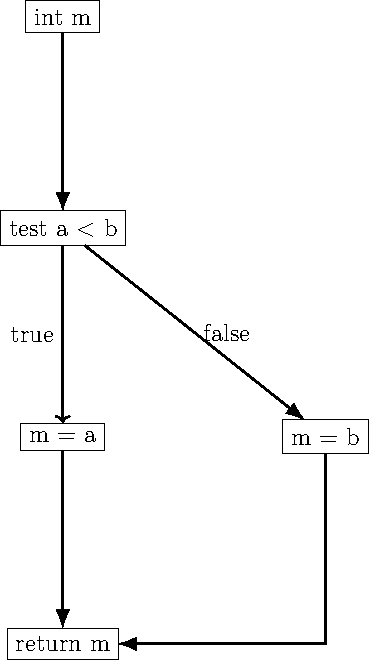
\includegraphics[width=5cm]{img/TP6/cfg_min.pdf} }}%
                \qquad
                \subfloat[\centering ]{{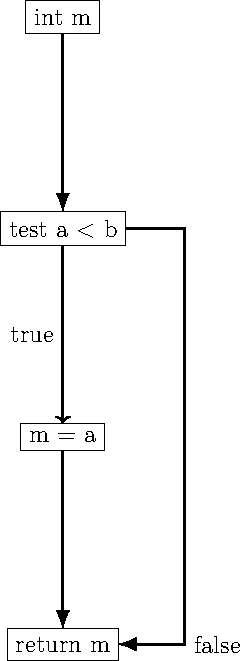
\includegraphics[width=5cm]{img/TP6/cfg_min_alternative.pdf} }}%
                \caption{CFG for min and minAlternative $(a|b|bc)^{*}a$}%
                \label{fig:example}%
            \end{figure}
    \addimg{img/TP6/cfg_squareSum.pdf}{scale=0.5}{CFG for squareSum}{}
    
    Non minimized SSA
    \begin{lstlisting}[language = Java , frame = trBL , firstnumber = last , escapeinside={(*@}{@*)}]
squareSum(n0):
    sum0 = 0
    i0 = 1
    goto loop(n0, sum0, i0)
loop(n1, sum1, i1):
    if i1<=n1 then goto body(n1,sum1,i1) else goto end(n1,sum1,i1)
body(n2, sum2, i2):
    t0 = i2*i2
    sum3 = sum2 + t0
    i3 = i2 + 1
    goto loop(n2, sum3, i3)
end(n3, sum4, i4):
    return sum4
\end{lstlisting}
    Minimized SSA
    \begin{lstlisting}[language = Java , frame = trBL , firstnumber = last , escapeinside={(*@}{@*)}]
squareSum(n0):
    sum0 = 0
    i0 = 1
    goto loop(sum0, i0)
loop(sum1, i1):
    if i1<=n0 then goto body else goto end
body:
    t0 = i1*i1
    sum3 = sum1 + t0
    i3 = i1+1
    goto loop(sum3, i3)
end:
    return sum1
\end{lstlisting}
    Non minimized non-SSA
    \begin{lstlisting}[language = Java , frame = trBL , firstnumber = last , escapeinside={(*@}{@*)}]
squareSum(n):
    sum = 0
    i = 1
    goto loop
loop:
    if i<=n then goto body else goto end
body:
    t = i*i
    sum = sum + t
    i = i +1
    goto loop
end:
    return sum
\end{lstlisting}
    Minimized non-SSA
    \begin{lstlisting}[language = Java , frame = trBL , firstnumber = last , escapeinside={(*@}{@*)}]
squareSum(n0):
    sum0 = 0
    i0 = 1
    sum1 = sum0
    i1 = i0
    goto loop
loop(sum1, i1):
    if i1<=n0 then goto body else goto end
body:
    t0 = i1*i1
    sum3 = sum1 + t0
    i3 = i1+1
    sum1 = sum3
    i1 = i3
    goto loop
end:
    return sum1
\end{lstlisting}

\subsection{Question 3}
    \textbf{Design a simple algorithm that verifies that a function has no missing return statement. The algorithm should also work for complex functions that contain many if-statements, loops, etc.}

    If you represent the start of the function and the end of the function as nodes in the control flow
graph, any path from the start node to the end node must contain a return statement.

